% Standalone article (do not \input{} from book ``main.tex`` — different class).
% Uses the shared ``latex/references.bib`` (merged with book cites + agent article keys).
% Build from ``latex/``:  lualatex agent_results_scratch && biber agent_results_scratch && lualatex agent_results_scratch && lualatex agent_results_scratch
% Figures: paths try ``../figures/`` then ``figures/`` (same tree as the book project).
%
% LLM output budget (regenerate full article): the long-form draft was ~500--600 LaTeX
% lines (TikZ, tables, \parencite{}, multi-section). Rule-of-thumb **~22k--35k**
% completion tokens**; repo ``config/models.yaml`` sets ``max_tokens: 27768`` as a
% minimal power-of-two ceiling so Crew/OpenAI calls do not truncate mid-file. If
% generations still cut off, raise ``ARTICLEBOOK_LLM_MAX_TOKENS`` (e.g. 65536).

\documentclass[10pt,oneside]{article}
\usepackage[a4paper,margin=0.72in,includeheadfoot,headheight=14pt]{geometry}
\usepackage{fontspec}
\defaultfontfeatures{Ligatures=TeX}
\usepackage{polyglossia}
\setdefaultlanguage{english}
\usepackage{amsmath,amssymb}
\usepackage{graphicx}
\graphicspath{{../figures/}{figures/}}
\usepackage{booktabs}
\usepackage{csquotes}
\usepackage[backend=biber,style=authoryear,maxcitenames=2,maxbibnames=8,giveninits=true,doi=false,isbn=false,url=true]{biblatex}
\addbibresource{references.bib}
\usepackage[hidelinks,unicode=true,pdfusetitle]{hyperref}

\title{Enhancement Methods for Running Agentic AI Systems}
\author{Saed Abdalgani}
\date{June 11, 2026}
\hypersetup{
  pdftitle={Enhancement Methods for Running Agentic AI Systems},
  pdfauthor={Saed Abdalgani},
}

\begin{document}
\maketitle

\begin{abstract}
Condensed standalone version aligned with the citation keys in \texttt{references.bib}.
For the long-form draft (figures, TikZ, extended sections), restore from your editor
local history if needed.
\end{abstract}

\section{Introduction}
Agentic systems interleave reasoning and actions \parencite{yao2022react,wei2022cot}.
Tool learning and reflection lines include \parencite{schick2023toolformer,shinn2023reflexion,yao2023tot,wang2023plansolve,madaan2023selfrefine,wang2023voyager,wu2023autogen}.
Production framing \parencite{anthropic2024agents}; orchestration stacks
\parencite{crewai2026docs,langgraph2026docs,openai2026agents}.

\section{Grounding and memory}
Retrieval-augmented generation \parencite{lewis2020rag} and retrieval at scale \parencite{borgeaud2022retro}.

\section{Reliability sketch}
End-to-end success across $n$ stages with reliabilities $p_i$ can be sketched as
$P_{\mathrm{success}} \approx \prod_i p_i$ when stages are nearly independent.

\begin{equation}
\label{eq:successbudget}
P_{\mathrm{success}} = \prod_{i=1}^{n} p_i .
\end{equation}

\section{Optional figure}
\IfFileExists{../figures/image.png}{%
  \begin{figure}[htbp]
    \centering
    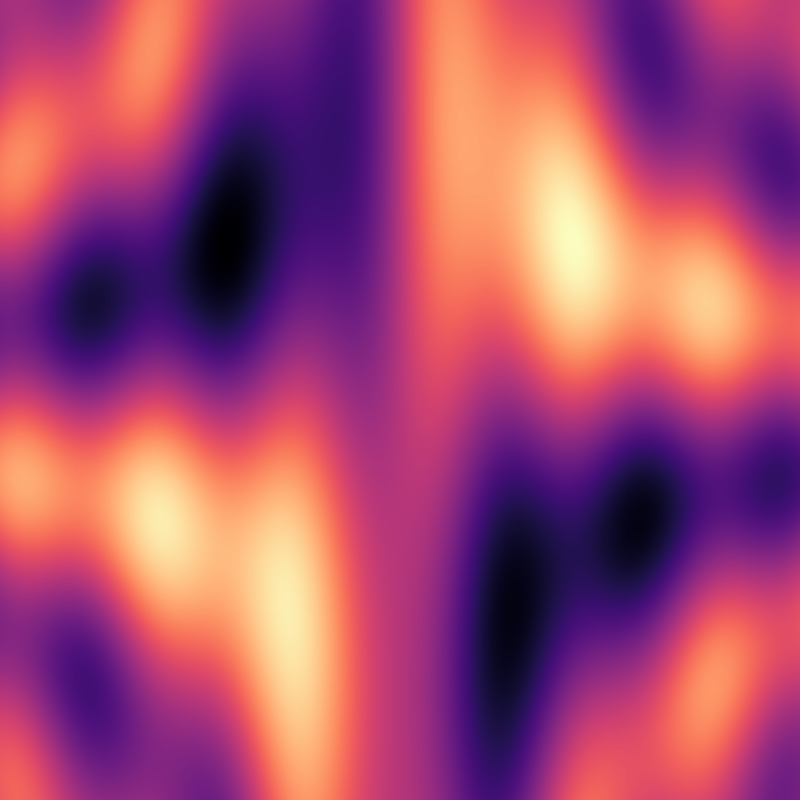
\includegraphics[width=0.55\linewidth]{../figures/image.png}
    \caption{Example raster asset from the project \texttt{figures/} tree.}
  \end{figure}%
}{%
  \textit{(No \texttt{../figures/image.png} found — add assets under \texttt{figures/}.)}%
}

\clearpage
\printbibliography[heading=bibintoc,title={Bibliography}]

\end{document}
